\documentclass[a4paper,10pt]{article}
\usepackage{amsmath}
\usepackage{amssymb}
\usepackage{mathtools}
\usepackage[all]{nowidow}
\usepackage{siunitx}
\usepackage{enumerate}

%Report-specific stuff
\usepackage{setspace}\doublespacing
\usepackage[margin=2.5cm]{geometry}

%Localisation
\usepackage{csquotes} %Context sensitive quotes: recommended by babel polyglossia
\usepackage[british]{babel}

\usepackage{titling}
%\setlength{\droptitle}{-0.5in} %Adjust margin above title

\usepackage{graphicx}
\usepackage[font=small,margin=0.45in]{caption}
\usepackage[labelformat=simple]{subcaption}
\usepackage{placeins} %Provides \FloatBarrier
\renewcommand\thesubfigure{(\alph{subfigure})}
%\usepackage{tikz}
%\usepackage{pgfplots}
\usepackage{float} %Provides the float option [H] for a non-floating float.
\graphicspath{{./figures/}}
\usepackage{flafter} %Floats come after the first reference to them.

%New Zealand Journal of Marine and Freshwater Research

\usepackage{xpatch}
\usepackage{hyperref}%Makes citations link to the bibliography.
\usepackage[backend=biber,style=authoryear-comp]{biblatex}

\ExecuteBibliographyOptions{sorting=ynt} %Year, name, title. Ensures that in-text citations are ordered chronologically.
\assignrefcontextentries[]{*} %Assigns all citations to the global refcontext, the sorting above.
%We will use a different refcontext around the bibliography to sort that by name.

\ExecuteBibliographyOptions{dashed=false} %Ensures that two papers by the same author are listed in full in the bibliography.
\ExecuteBibliographyOptions{maxbibnames=10,minbibnames=10} %In the bibliography, the first maxnames authors are listed, then the list is truncated to minnames
\ExecuteBibliographyOptions{maxcitenames=2,mincitenames=1} %In-text, two authors are listed in full, three or more are first author then et al.
\ExecuteBibliographyOptions{citetracker=true} %For use in line below.
%\AtEveryCitekey{\ifciteseen{}{\defcounter{maxnames}{3}\clearfield{namehash}}}%Three names before andothers on first citation.
%TODO: Check letters after year for multiple papers by same author in same year.

%\ExecuteBibliographyOptions{uniquename=false,uniquelist=false}%Disables disambiguation that would violate the min/max names above.
\ExecuteBibliographyOptions{giveninits=true} %Initialises all given names.
\ExecuteBibliographyOptions{terseinits=true} %Removes periods and spaces around initials
\ExecuteBibliographyOptions{doi=false, eprint=false, url=false, isbn=false}

\DeclareNameAlias{author}{last-first} %Ensures all authors are given as "surname, given initials", rather than "given initials surname".
\DeclareNameAlias{sortname}{last-first} %Ditto for everything else
\DeclareNameAlias{default}{last-first}

\AtEveryBibitem{\clearfield{number}} %Removes issue numbers, but leaves volume numbers.
\AtEveryBibitem{\clearfield{month}} %Removes month of publication.
\AtEveryBibitem{\clearfield{note}} %Removes the `note' field.

%\xpatchbibmacro{name:andothers} {\bibstring{andothers}} {\bibstring[\textit]{andothers}} {}{}%Italicises et al.

%Remove `In:' before the journal title for articles, but keeps it for other entries.
\xpatchbibdriver{article}{%
	\usebibmacro{in:}%
}{%
	%Just delete it; replace it with nothing.
}{}{}

\DeclareFieldFormat[article]{pages}{#1} %Removes pp. or p. from article pages ranges.
\DeclareFieldFormat[article,inproceedings,inbook,thesis]{title}{#1} %Removes quotes around article/chapter/thesis title.

%Add a comma after the journal title for articles.
\xpatchbibmacro{journal+issuetitle}{%
	\usebibmacro{journal}%
	\setunit*{\addspace}%
}{%
	\usebibmacro{journal}%
	\setunit*{\addcomma\addspace}%
}{}{}

%Swap so that publisher comes *before* location.
\xpatchbibmacro{publisher+location+date}{%
	\printlist{location}%
	\iflistundef{publisher}
		{\setunit*{\addcomma\space}}
		{\setunit*{\addcolon\space}}%
	\printlist{publisher}%
}{%
	\printlist{publisher}%
	\iflistundef{location}
		{}
		{\setunit*{\addcomma\space}}%%
	\printlist{location}%
}{}{}

%TODO: Test and if necessary correct handling of book editions numbers.
%See https://onlinelibrary.wiley.com/doi/epdf/10.1111/ele.13171 for handling in existing paper.

%Only print the book subtitle punctuation if there's a subtitle.
\xpatchbibmacro{booktitle}{%
	\setunit{\subtitlepunct}%
	\printfield[titlecase]{booksubtitle}%
}{%
	\iffieldundef{booksubtitle}
	{}
	{%
		\setunit{\subtitlepunct}%
		\printfield[titlecase]{booksubtitle}%
	}%
}{}{}

%Remove the extra period that gets forced in after the booktitle, allowing the bibdrivers to handle it properly.
\xpatchbibmacro{booktitle}{%
	\newunit
}{%
	%Just delete it; replace it with nothing.
}{}{}
%Ditto; remove the extra period.
\xpatchbibmacro{maintitle+booktitle}{%
	\usebibmacro{booktitle}%
	\newunit%
}{%
	\usebibmacro{booktitle}%
}{}{}

%Remove period between book title and editors.
\xpatchbibdriver{inbook}{%
	\usebibmacro{maintitle+booktitle}%
	\newunit\newblock
	\usebibmacro{byeditor+others}%
}{%
	\usebibmacro{maintitle+booktitle}%
	{\setunit*{\space}}
	\usebibmacro{byeditor+others}%
}{}{}
%As above, for inproceedings.
\xpatchbibdriver{inproceedings}{%
	\usebibmacro{maintitle+booktitle}%
	\newunit\newblock
	\usebibmacro{event+venue+date}%
	\newunit\newblock
	\usebibmacro{byeditor+others}%
}{%
	\usebibmacro{maintitle+booktitle}%
	%{\setunit*{\space}}
	%\usebibmacro{event+venue+date}%Have to knock this out to get no period between booktitle and editors. TODO: Check this is okay.
	%{\setunit*{\space}}\newblock
	\usebibmacro{byeditor+others}%
}{}{}

%Wrap the editor info in parentheses. Use the correct editor string.
\renewbibmacro*{byeditor+others}{%
	\ifboolexpr{
		test {\ifnameundef{editor}}
		and
		test {\ifnameundef{editora}}
		and
		test {\ifnameundef{editorb}}
		and
		test {\ifnameundef{editorc}}
		and
		test {\ifnameundef{translator}}
		and
		test {\ifnameundef{commentator}}
		and
		test {\ifnameundef{annotator}}
		and
		test {\ifnameundef{introduction}}
		and
		test {\ifnameundef{foreword}}
		and
		test {\ifnameundef{afterword}}
	}
	{} %If we'd be printing no names at all, don't bother with the parentheses.
	{
		\printtext[parens]{%
			\ifnameundef{editor}
				{}
				{\usebibmacro{editorstrg}%This is also changed, from `byeditor+othersstrg'.
				\setunit{\addspace}%
				\printnames[byeditor]{editor}%
				\clearname{editor}%
				\newunit
			}%
			\usebibmacro{byeditorx}%
			\usebibmacro{bytranslator+others}%
		}%
	}%
}

%TODO: Check book and inbook format. Article and inproceedings should be okay.

%Ensure proper citation of Dutch names:
%https://en.wikipedia.org/wiki/Van_(Dutch)#Collation_and_capitalisation

\ExecuteBibliographyOptions{useprefix=true} %Make sure it actually picks up the prefixes.

\AtBeginDocument{%
	\renewcommand*{\mkbibnameprefix}[1]{\MakeCapital{#1}} %Capitalise prefixes in citations.
}
\AtBeginBibliography{%
	\renewcommand*{\mkbibnameprefix}[1]{#1} %But not in the bibliography
}

\renewbibmacro*{begentry}{\midsentence} %Begin bibliography entries midsentence, such that there is no capitalisation of van.

\DeclareSortingNamekeyScheme{ %Sort by family name, then by prefix. So van Gardingen sorts under G, not v.
	\keypart{
		\namepart{family}
	}
	\keypart{
		\namepart{prefix}
	}
	\keypart{
		\namepart{given}
	}
	\keypart{
		\namepart{suffix}
	}
}

%Join to authors with an ampersand, not 'and'
%\renewcommand*{\finalnamedelim}{\addspace\&\addspace}

%Remove the comma betwen the surname and the initials
\renewcommand*{\revsdnamepunct}{}

%Remove all italics from the bibliography with a nasty hack:
%There are some options we only want to apply in the bibliograph, so here's a nasty hack.
\let\printinnerbibliography\printbibliography %Copy the original command so we can modify it
\renewcommand{\printbibliography}{
	\begingroup
	\let\itshape\upshape %Remove all italics
	\renewcommand*{\finalnamedelim}{\addcomma\addspace} %Remove 'and' between penultimate and ultimate author
	\begin{refcontext}[sorting=nyt]%Sorts the bibliography by name, then year, then title.
		\printinnerbibliography
	\end{refcontext}
	\endgroup
}

\addbibresource{report.bib}

\let\dotlessi\i %Copy the definition so we can safely redefine \i
\newcommand\naive{na\"{\dotlessi}ve}
\newcommand\Naive{Na\"{\dotlessi}ve}

\newcommand\norm[1]{\left\lVert#1\right\rVert}
\newcommand\abs[1]{\left\lvert#1\right\rvert}
\renewcommand{\d}{\mathrm{d}}
\newcommand{\D}[1]{\mathop{\d #1}}
\renewcommand{\i}{\mathrm{i}}
\newcommand{\e}{\mathrm{e}}
\newcommand{\Imat}{\mathrm{I}}
\newcommand{\bigO}{\mathcal{O}}
\newcommand{\transpose}[1]{{#1}^{\mathrm{T}}}

%Have to delete existing commands first.
\let\Re\relax
\let\Im\relax
\DeclareMathOperator{\Re}{Re}
\DeclareMathOperator{\Im}{Im}
\DeclareMathOperator{\trace}{tr}
\DeclareMathOperator{\J}{J}

\newcommand\inputresults[1]{\input{results/#1}\unskip}

%Custom commands
\usepackage{suffix}%includes \WithSuffix
\newcommand\spbinom[1]{%
	\emph{#1}%
}
\WithSuffix\newcommand\spbinom*[1]{%
	\StrCut{#1}{}{\genus}{\species}%
	\emph{\StrLeft{\genus}{1}. \species}%
}

\newcommand\datadate{5 September 2019} %The date the fieldwork was performed on.

\title{A Comparison of Macroinvertebrate $\alpha$- and $\beta$-Diversity in Disturbed and Stable Streams}
\author{
	Christopher Brown\\15413822
}
\date{}

\begin{document}
\maketitle

\begin{center}
	\emph{Word Count}: %TODO
\end{center}

\section*{Abstract}

The effect of disturbance upon $\alpha$-diversity has been debated for many years, focussing upon the intermediate disturbance hypothesis.
The effect upon $\beta$-diversity has only been studied more recently, with conflicting results.
Disturbance may homogenise communities through species filtering or diversify them by allowing stochastic colonisation.

We studied diversity of freshwater macroinvertebrates across a stream disturbance gradient in Canterbury, New Zealand.
We found that disturbance caused a monotonic reduction of $\alpha$-diversity and a shift in community composition, but had no significant effect on $\beta$-diversity.
We posit that this is a result of both species filtering and stochastic colonisation acting in opposition to one another.

\bigskip\noindent\emph{Keywords}:
beta diversity,
biodiversity,
freshwater macroinvertebrates,
New Zealand,
disturbance
%TODO: Keywords

\clearpage

\section*{Introduction}

The relationship between disturbance and biodiversity is an important but hotly contested topic in ecology.
The intermediate disturbance hypothesis (IDH) posits that biodiversity will be highest with an intermediate level of disturbance: too much disturbance is unsurvivable for most species, but too little leads to a small handful of species competitively excluding all others \parencite{idh-original}.
Since its original formulation, the hypothesis has been subject to innumerable studies \parencite{disturbance-diversity-predict-test}.
Great swathes of evidence have fallen both in support of and against the IDH, and papers have called for both its abandonment \parencite{idh-abandon} and its more widespread use \parencite{idh-patch-dynamics}.

Even in studies of very similar systems, New Zealand freshwater benthic macroinvertebrates, results have differed.
\textcite{idh-refugia-streams}, sampling in Otago, found precisely the pattern predicted by the IDH, while \textcite{diversity-stability-canterbury}, in Canterbury, found a simple monotonic decrease of diversity with increasing disturbance.

The IDH pertains only to $\alpha$-diversity, however; the relationship between disturbance and $\beta$-diversity is less well studied.
Positive and negative effects of disturbance on $\beta$-diversity have both been hypothesised:
disturbance may reduce $\beta$-diversity through uniformly removing taxa that are not resistant or resilient to disturbance, homogenising communities,
or it may increase $\beta$-diversity, replacing deterministic dominance by the competitively superior species with the stochastic process of colonisation \parencite{disturbance-beta-meta}.
Both responses have been observed empirically \parencite{disturbance-increase-beta, homogenisation-agriculture}, and meta-analysis has yielded no conclusive results \parencite{disturbance-beta-meta}.

To provide another test of the effects of disturbance upon $\beta$-diversity, as well as $\alpha$-diversity and community composition, we studied freshwater macroinvertebrate communities across a disturbance gradient in ten waterways in the Cass region of Canterbury, New Zealand.

\section*{Methods}

Ten waterways around the Cass region of Canterbury, New Zealand were selected for the study.
Five were braided rivers, highly disturbed.
The other five were more stable spring-fed streams.
To confirm this intuition, we assessed the Pfankuch Stability Score of each stream \parencite{pfankuch, pfankuch-doc}.
The Pfankuch scores of the ten streams divided them clearly into a stable and a disturbed cluster, exactly as predicted (Figure \ref{fig:regressions}).
As such, we remained confident in treating disturbance categorically through the permutational tests.

At each waterway, a kick net sample of macroinvertebrates was taken.
Sampling occurred at five points inside each stream, selected by eye to be as diverse as possible within the reach.
All five samples per stream were combined in the same net.
Samples were bagged with water and live-picked later the same day.

To keep sampling time reasonable, abundances were recorded semi-quantitatively according to the same coded-abundance categories as used in calculating \possessivecite{sqmci} Semi-Quantitative Macroinvertebrate Community Index (SQMCI):
0, 1--4, 5--19 and 20--99 (nothing above this range was observed).
For coded abundance analyses, as in SQMCI, results were treated as though they lay at the bottom of the interval.
Stoneflies, mayflies and caddisflies were resolved to the genus level; other taxa were resolved between the phylum and genus level, as far as possible.

To examine the effect of stream disturbance upon $\alpha$-diversity, we performed two generalised linear regressions: taxonomic richness and total coded abundance of each stream as a function of the Pfankuch score.
Due to the count nature of the data and under- and over-dispersion in Poisson regression, we used quasi-Poisson regression.

In order to help explain any changes in community composition that might be observed, a third generalised linear regression (binomial) examined the proportion of macroinvertebrates which had a shell or case, again as a function of the Pfankuch score.
It is worth noting that this was not actually a true proportion due to the semi-quantitative nature of the abundances (simply the total coded abundance of cased and shelled taxa divided by the total coded abundance of all taxa).

For the remainder of the analyses, a dissimilarity was calculated between each pair of sites.
To make full use of the collected semi-quantitative (ordinal, partially ranked) data, we used the Hausdorff extension of an edit distance metric, as developed by \textcite{critchlow} and recommended by \textcite{dissimilarity-partially-ranked}.
In particular, we used Kendall's tau, reasoning that ecological gradients were more likely to cause shifts in the relative abundances of species than immediate wholesale removals (as in Ulam's metric) or substitutions (as in Hamming's distance).
An edit distance between rankings, where absent species are also ranked (tied for the lowest rank, coded abundance 0), should provide a measure of $\beta$-diversity that remains independent of $\alpha$-diversity.
%TODO: Address concerns from dissimilarity-partially-ranked about using low values as much as high values: we won't fall on both sides of the mode as we seem to have a linear gradient (no IDH).

From the distance matrix, we created an ordination plot using classical multidimensional scaling.
We tested for differences in community composition between the disturbed and stable streams using a permutational multivariate ANOVA.
We used community dispersion as a measure of $\beta$-diversity \parencite{dispersion-diversity} and tested for differences using \possessivecite{permdisp2} permutation test.
All analyses were performed using \texttt{R}, with the \texttt{vegan} package \parencite{vegan} for the permutation tests.

%TODO: GitHub

\section*{Results}

According to the Pfankuch scores, the sampled waterways ran nearly the full gamut of disturbance.
The score ranges from 38 to 152, and the sampled streams ranged from 47 to 125.
Stable streams always exhibited abundant macrophyte life, while the disturbed waterways, the braided rivers, had essentially no vegetation below the upper banks.

26 different taxa were observed in total, many in only one stream and some only once.
One taxon, however, the mayfly genus \spbinom{Deleatidium}, was present in every stream sampled.
Several taxa only appeared in the stable streams, such as the mayfly \spbinom{Nesameletus}, the cased caddisfly \spbinom{Olinga} the snail \spbinom{Potamopyrgus}.

%TODO: More general observations.
%Abundance and richness? Or just point to the figure for these?

As the stability of the studied streams increased (as the Pfankuch score decreased), there was a clear, monotonic, more than two-fold increase of both macroinvertebrate abundance (\inputresults{abundance-regression}) and taxonomic richness (\inputresults{richness-regression}) (Figure \ref{fig:regressions}).

The site ordination is shown Figure \ref{fig:site-ordination}.
There was no difference in community dispersion between the stable and the disturbed streams (\inputresults{permdisp}), but the community compositions differed significantly (\inputresults{permanova}).
%TODO: Report the correct things for PERMANOVA and PERMDISP.

There was a significant decrease in the proportion of shelled macroinvertebrates with increasing Pfankuch score (\inputresults{shell-abundance-regression}; Figure \ref{fig:shell-abundance-regression}).
Although this was not a true proportion, the trend was plain.
In fact, no disturbed stream had more than one cased or shelled taxon, or more than the lowest abundance code for its one taxon.
Meanwhile, every stable spring had at least 20 cased or shelled individuals.

\section*{Discussion}

Our data showed no evidence in support of the intermediate disturbance hypothesis.
$\alpha$-diversity increased monotonically with increasing stability, agreeing entirely with the results of \textcite{diversity-stability-canterbury}, who also studied freshwater macroinvertebrates in the Cass region.
It is worth noting that, due to the selection of either stable or disturbed streams, there is a gap with no sites at a very intermediate disturbance.
However, the small relative width of the gap and the very linear relationship of the sampled sites strongly suggests that there is no intermediate hump.

One way in which a study may fail to find evidence of the IDH is that the sampled range of their predictor variable was insufficient to encompass the diversity peak.
To be the case here, the peak would have to lie at a more stable stream than any we sampled.
We find that unlikely to be the case here, as the stable streams were very low-order, spring-fed streams, and reached very nearly to the bottom of the Pfankuch scale; more stable streams could barely exist.

A likely reason for the observed pattern of $\alpha$-diversity lies in the fact that increasing disturbance in the studied streams was accompanied by decreasing habitat heterogeneity.
Stable streams contained abundant macrophytes, while the disturbed streams were bare, rocky braided riverbeds.
Diverse macrophytes are essential to provide the habitat for a diverse community of macroinvertebrates \parencite{macrophyte-associations}.
Moreover, the increased habitat heterogeneity may help to avoid the competitive exclusion the IDH posits in stable environments, due to niche partitioning \parencite{heterogeneity-competition,idh-patch-dynamics}. %TODO: A better citation.

We observed a significant shift in community composition between the disturbed and stable streams.
This is no great surprise; its seems as though every study of community composition under disturbance has seen the same result \parencite{disturbance-composition-invasion, disturbance-composition-simulate, disturbance-composition-desert, meta-richness-disturbance}.
This might reflect species filtering caused by the disturbance, where less resistant and resilient species are filtered out of the disturbed streams.
We see direct evidence of such filtering in the loss of shelled and cased invertebrates in the disturbed streams; these species cannot typically tolerate flood events \parencite{flood-braided-river, flood-community-composition}.
This might homogenise the disturbed streams, in turn decreasing their $\beta$-diversity \parencite{disturbance-beta-meta}.

However, this result may instead reflect standard changes along a stream's length, per the River Continuum Concept \parencite{rcc}.
The disturbed streams were overall larger and unvegetated, while the stable ones were smaller, lower-order streams with abundant riparian and aquatic vegetation.
As such, we would expect differences in their communities due to this alone, such as a higher proportion of shredding macroinvertebrates in the vegetated streams \parencite{rcc}.

We observed no significant change in community dispersion, $\beta$-diversity, between disturbed and stable streams.
This is perhaps unsurprising, considering that there are proposed mechanisms by which disturbance might influence $\beta$-diversity in both directions.
Indeed, a meta-analysis by \textcite{disturbance-beta-meta} found no consistent, significant effect in either direction.
Our result implies that either both mechanisms (homogenisation due to species filtering and diversification due to stochastic colonisation) were acting in opposition to one another, or that neither is acting particularly strongly.
The change in community composition, and the fact that there were several species present only in the stable streams (particularly cased and shelled species) suggests that species filtering seemed to be occurring.
Hence, both mechanisms were probably in force.

Overall, we have observed several important effects of disturbance on the streams' macroinvertebrate communities.
It applies a species filter, reducing $\alpha$-diversity and shifting the community composition.
But our data also suggest that such filtering can free space in the disturbed streams for stochastic colonisation by species that might not otherwise be present, preventing a loss of $\beta$-diversity.

\section*{Acknowledgements}

Thanks to the University of Canterbury for the use of the Cass field station.
Thanks to Delia Teesdale and Chynae Stark for help in data collection, and to Linda Morris for fieldwork logistics.
Thanks to Angus McIntosh, Jon Harding and Helen Warburton for advice on experimental design and general education.
And thanks to Eva Delmas for directing me to the paper that finally unravelled the mystery of how to analyse semi-quantitative multivariate data.

\FloatBarrier
\printbibliography

\clearpage

\begin{figure}[p]
	\centering
	\begin{subfigure}[t]{\textwidth}
		\centering
		\includegraphics[width=\textwidth]{abundance-regression}
		\caption{}\label{fig:abundance-regression}
	\end{subfigure}
	\begin{subfigure}[t]{\textwidth}
		\centering
		\includegraphics[width=\textwidth]{richness-regression}
		\caption{}\label{fig:richness-regression}
	\end{subfigure}
	\begin{subfigure}[t]{\textwidth}
		\centering
		\includegraphics[width=\textwidth]{shell-abundance-regression}
		\caption{}\label{fig:shell-abundance-regression}
	\end{subfigure}
	\caption[Regression plots]{ %[] provides a caption for the table of contents, allowing paragraph breaks in the full caption.
		Scatterplots showing the total coded abundance \subref{fig:abundance-regression}, taxonomic richness \subref{fig:richness-regression} and proportion of shelled or cased individuals \subref{fig:shell-abundance-regression} for macroinvertebrates over a stream disturbance gradient around Cass, Canterbury.
		A higher Pfankuch score indicates a more disturbed stream.
		Note that the proportion is not a true proportion, as it is calculated from semi-quantitative data.
		Generalised linear regression lines with \SI{95}{\percent} confidence intervals are also shown: quasi-Poisson for \subref{fig:abundance-regression} and \subref{fig:richness-regression}, binomial for \subref{fig:shell-abundance-regression}.
		Data gathered {\datadate}.
	}\label{fig:regressions}
\end{figure}

\begin{figure}[p]
	\centering
	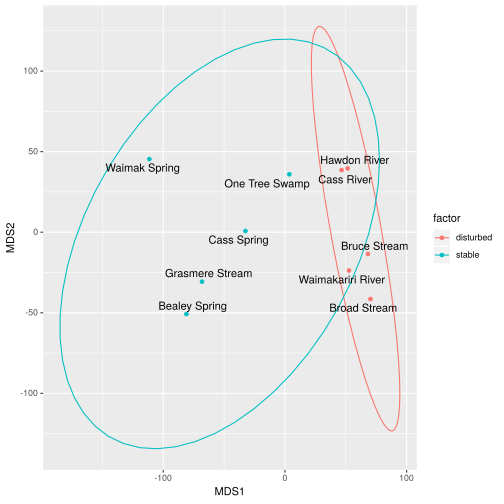
\includegraphics[width=\textwidth]{site-ordination}
	\caption[Site ordination]{ %[] provides a caption for the table of contents, allowing paragraph breaks in the full caption.
		An ordination (metric multidimensional scaling) of macroinvertebrate community composition in streams around Cass, Canterbury.
		\SI{95}{\percent} normal confidence ellipses are also shown.
		Based upon semi-quantitative coded abundance data, with site-site distances defined by the Hausdorff extension of Kendall's tau metric.
		Produced using the \texttt{cmdscale} function in \texttt{R}.
		Data gathered {\datadate}.
	}\label{fig:site-ordination}
\end{figure}

%TODO: Do CI ellipses make sense in MDS?

\end{document}
